\documentclass[border=10pt]{standalone}
\usepackage{tikz}
\usetikzlibrary{arrows.meta}

% ========== 颜色：20层蓝 / 56层红 ==========
\colorlet{c20}{blue!70!black}
\colorlet{c56}{red!70!black}

\begin{document}
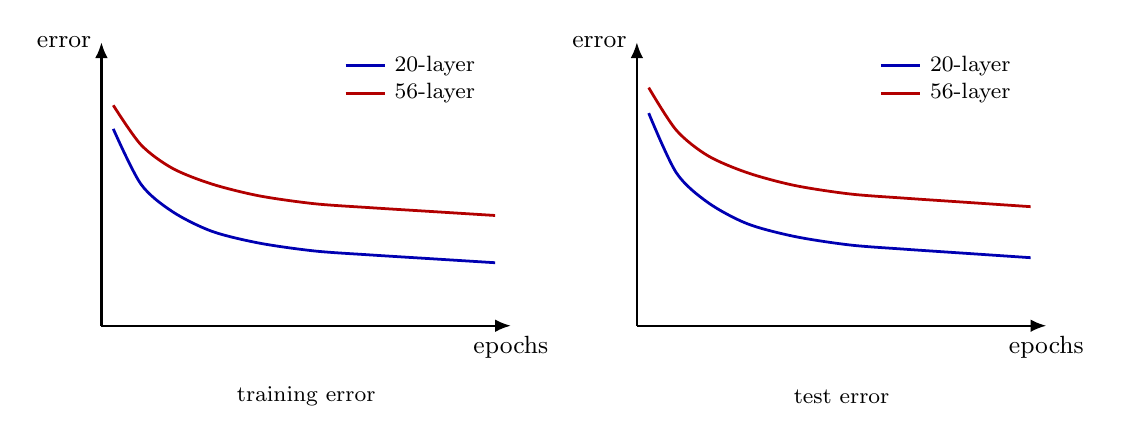
\begin{tikzpicture}[
    font=\small,
    >={Latex[length=2mm, width=1.6mm]},
    axis/.style={->, line width=.8pt},
    curve/.style={line width=1pt, smooth}
  ]

  % ========== 面板宏：#1=横向位置 #2=标题 #3=纵向缩放 ==========
  \newcommand{\panel}[3]{%
    \begin{scope}[xshift=#1]
      % 坐标轴
      \draw[axis] (0,0) -- (5.2,0)  node[below] {epochs};
      \draw[axis] (0,0) -- (0,3.6) node[left]  {error};
      % 20 层（蓝，较低）
      \draw[curve, c20] plot coordinates {
        (0.15,{2.5*#3}) (0.5,{1.8*#3}) (0.9,{1.45*#3}) (1.4,{1.2*#3})
        (2.0,{1.05*#3}) (2.7,{.95*#3}) (3.4,{.9*#3}) (4.2,{.85*#3}) (5,{.8*#3})};
      % 56 层（红，较高：训练误差也更大 => 非过拟合）
      \draw[curve, c56] plot coordinates {
        (0.15,{2.8*#3}) (0.5,{2.3*#3}) (0.9,{2.0*#3}) (1.4,{1.8*#3})
        (2.0,{1.65*#3}) (2.7,{1.55*#3}) (3.4,{1.5*#3}) (4.2,{1.45*#3}) (5,{1.4*#3})};
      % 图例
      \draw[curve, c20] (3.1,3.3)--(3.6,3.3);
      \node[right, font=\footnotesize] at (3.6,3.3) {20-layer};
      \draw[curve, c56] (3.1,2.95)--(3.6,2.95);
      \node[right, font=\footnotesize] at (3.6,2.95) {56-layer};
      % 面板标题
      \node[font=\footnotesize] at (2.6,-0.9) {#2};
    \end{scope}
  }

  % ========== 两个面板 ==========
  \panel{0cm}{training error}{1}
  \panel{6.8cm}{test error}{1.08}

\end{tikzpicture}
\end{document}